\documentclass[letterpaper,12pt,oneside]{book}
%\usepackage[a4paper,includeall,bindingoffset=0cm,margin=2cm,marginparsep=0cm,marginparwidth=0cm]{geometry}
\usepackage[top=1in, left=0.9in, right=1.25in, bottom=1in]{geometry}
\usepackage{bachelorstitlepageUNAM}
\usepackage[utf8]{inputenc}
%%%%%%%%%%%%%%%%%%%%%%%%%%%%%
% Comparto una plantilla para la PORTADA que us\'e en mi t\'esis
% basada en el dise\~no gen\'erico que se usa en la Facultad de Ciencias
% Para usarlo \'unicamente aseg\'urate de tener la l\'inea
% \usepackage{bachelorstitlepageUNAM} y el archivo bachelorstitlepageUNAM.sty en el mismo directorio de trabajo.
% y los campos (sin signo %) :
%\author{Nombre del Alumno}
%\title{T\'itulo de la tesis}
%\faculty{Facultad}
%\degree{Grado que obtienes}
%\supervisor{ Tutor}
%\cityandyear{Ciudad y anio}
%\logouni{nombredelescudodelaunamsinespacios}
%\logofac{NombreDeLaImagenDelEscudodeTuFacultadSinEspacios}
% Para sugerencias y comentarios: DM en twitter.com/sglvgdor
% Subir\'e mas adelante la plantilla para maestr\'ia
%%%%%%%%%%%%%%%%%%%%%%%%%%%%%

%\author{Irving Yosafat Angel Camacho}
%\title{Métodos Numéricos de la Hidrodinámica Relativista aplicados a problemas de acreción y eyección en %jets astrofísicos}
%\faculty{Escuela Nacional de Estudios Superiores\\
%            Unidad Morelia}
%\degree{Licenciado en Geociencias}
%\supervisor{Dr. Sergio Mendoza Ramos \\ 
%Dr. Sinhué A. R. Haro Corzo}
%\cityandyear{Morelia, Michoacán, 2019}
%\logouni{Escudo-UNAM}
%\logofac{logo-enes}
%
%-------------------------------

%###################################
% Artículo 12.- El protocolo de tesis, con el visto bueno de un asesor, deberá ser entregado por 
% el alumno a la Coordinación de Carrera correspondiente para su registro, así como para su 
% presentación ante el Comité de Aprobación de Protocolo de Tesis correspondiente. El alumno 
% deberá tener un mínimo del 90% de créditos de su carrera para registrar su protocolo. La 
% Coordinación de Carrera será la responsable de realizar las gestiones académico-administrativas de 
% esta opción de titulación.
% Para someter el protocolo de tesis al Comité de Aprobación de Protocolo de Tesis respectivo, se 
% deberá entregar un documento que no exceda de cinco cuartillas, además de la portada, 
% considerando el contenido siguiente:
%    a) Portada, la cual deberá incluir: título del trabajo de tesis, nombre del alumno y nombre del asesor;
%    b) Objetivo(s) del trabajo;
%    c) Índice tentativo del trabajo de tesis;
%    d) Introducción, antecedentes y justificación del trabajo;
%    e) Metodología a emplear, y
%    f) Bibliografía básica (mínimo 10 referencias)
%###################################
\usepackage{float}
\newcommand{\figura}[4]
{
  \begin{figure}[H]
    \centering
    \includegraphics[scale=#1]{#2}
    \caption{#3}
    \label{#4}
  \end{figure}
}
\newcommand{\refig}[1]{\figurename~\ref{#1}}
\newcommand{\reteo}[1]{$\mathfrak{Teorema}$~\ref{#1}}
\newcommand{\bb}[1]{\{#1\}}

%%Definiciones matemáticas
%\newtheorem{defi}{{\it Definici\’on}}[chapter]
\newtheorem{defi}{\textit{\textmd{$\mathfrak{Definición}$} }}
\newtheorem{teo}{\textit{\textmd{$\mathscr{TEOREMA}$} }}


%-----------------------__--------

\usepackage[T1]{fontenc}
\usepackage[utf8]{inputenc}
\usepackage[spanish,es-nodecimaldot,es-tabla]{babel}
\usepackage{graphicx}
\usepackage{tikz} 
\usepackage{tocloft}
\graphicspath{{./figs/}}
\usepackage{setspace}
\usepackage[nottoc]{tocbibind}
%\usepackage[round]{natbib}

\renewcommand\cftsecpresnum{\S}
\renewcommand\cftsubsecpresnum{\S}   


\begin{document}
%------------------------------

    \begin{titlepage}
        \thispagestyle{empty}
        \begin{minipage}[c][0.17\textheight][c]{0.25\textwidth}
            \begin{center}
                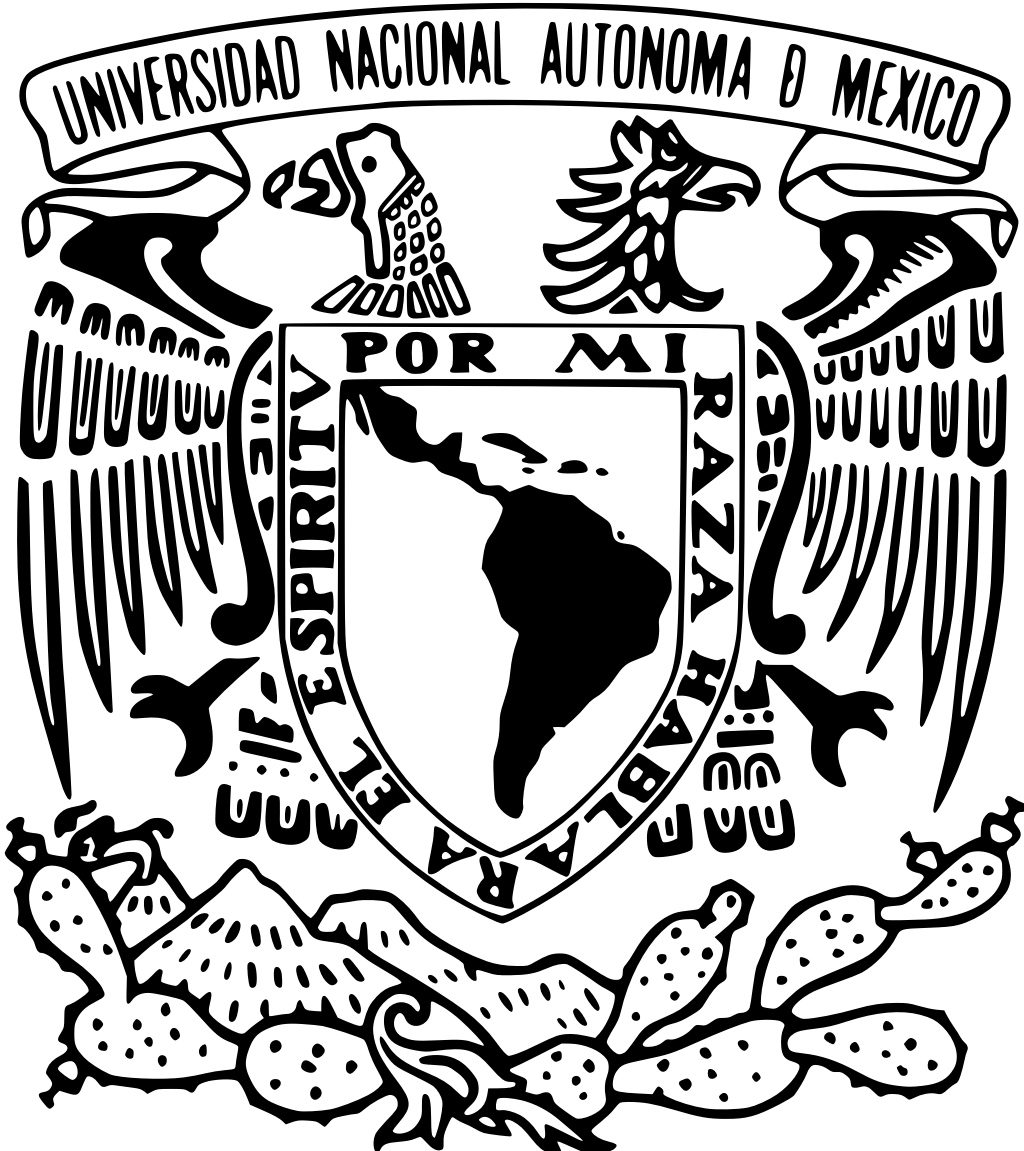
\includegraphics[width=3.5cm, height=3.5cm]{/home/aceron/Documentos/GitHub/Tesis/docTesis/Escudo-UNAM.png}
            \end{center}
        \end{minipage}
        \begin{minipage}[c][0.195\textheight][t]{0.75\textwidth}
            \begin{center}
                \vspace{0.3cm}
                \textsc{\large Universidad Nacional Aut\'onoma de M\'exico}\\[0.5cm]
                \vspace{0.3cm}
                \hrule height2.5pt
                \vspace{.2cm}
                \hrule height1pt
                \vspace{.8cm}
                \textsc{CENTRO DE FÍSICA APLICADA Y TECNOLOGÍA AVANZADA}\\[0.5cm] %
            \end{center}
        \end{minipage}

        \begin{minipage}[c][0.81\textheight][t]{0.25\textwidth}
            \vspace*{5mm}
            \begin{center}
                \hskip2.0mm
                \vrule width1pt height13cm 
                \vspace{5mm}
                \hskip2pt
                \vrule width2.5pt height13cm
                \hskip2mm
                \vrule width1pt height13cm \\
                \vspace{5mm}
                
\includegraphics[height=4.0cm]{/home/aceron/Documentos/GitHub/Tesis/docTesis/Esculo-CFATA.png}
            \end{center}
        \end{minipage}
        \begin{minipage}[c][0.81\textheight][t]{0.75\textwidth}
            \begin{center}
                \vspace{1cm}

                {\large\scshape (Título tentativo) Estudio de la viabilidad de sistemas de recolección de agua de lluvia en el Estado de Querétaro usando datos del radar meteorológico ubicado en el Cerro de la Ronchera}\\[.2in]

                \vspace{2cm}            

                %\textsc{\LARGE T\hspace{1.5cm}E\hspace{1.5cm}S\hspace{1.5cm}I\hspace{1.5cm}S}\\[0.5cm]
                %\textsc{\large que para obtener el t\'itulo de:}\\[0.5cm]
                %\textsc{\large Licenciado en Tecnología}\\[0.5cm]
                \textsc{\large Protocolo de Tesis}\\[0.5cm]
                \textsc{\large presenta:}\\[0.5cm]
                \textsc{\large {Ariel Cerón González}}\\[2cm]          

                \vspace{0.5cm}

                {\large\scshape Tutores:\\[0.3cm] {Dr. Adolfo Magaldi Hermosillo}}\\[.2in]

                \vspace{0.5cm}

                \large{Querétaro, Querétaro}{ }{2021}
            \end{center}
        \end{minipage}
    \end{titlepage}



%---------------------------------
\frontmatter
%\maketitle
% \chapter*{}
% \begin{flushright}%
%   \emph{Dedicatoria ...}
%   \thispagestyle{empty}
% \end{flushright}

% \chapter{Agradecimientos}
% \spacing{1.5}%\doublespacing

%\chapter{Notación}

\chapter{Introducción}
    En México, el manejo de los recursos hídircos es uno de los grandes temas de interes para diferentes sectores plitico-industriales, por el beneficio económico que genera. 

    Actualmente México enfrenta varias problemática sobre el recurso entre las que se encuentran el acceso al recurso, mala calidad en el suministro, la falta de lluvias originado por la tala inmoderada de bosques y selvas, sobre consesiones del recurso\cite{jornada:agua}, y falta de matenimiento a la infraestrucutra existente.

    Aunque en los últimos años se ha reconocido la importancia de cuidar y administrar el recurso \cite{de2019objetivo} \cite{mex:procaptar} son pocas las nuevas tecnologías o métodos que se han desarrollado para la solución del problema. Una de las soluciones que más destaca es la de la captación del agua de lluvia \cite{comision2016lineamientos} \cite{hugues2019captacion} \cite{nickisch2018sistemas} \cite{van2013captacion} sin embargo las soluciones no consideran aspectos meteorológicos para su aplicación, sino que se realizan mediciones \textit{in situ} para validar la eficiencia del sistema.

    El aprovechamiento de tecnologías meteorológicas, como el radar, podrían dotar de más información que permita validar la eficiencia de sistemas, como el de capatación, sin la necesidad de realizar una instalación, ahorrando costos en la implementación del sistema o, por otro lado, eficientizandolos, además los resultados pueden ser considerados para la implementación de mejores politicas de gestión pública del recurso.
\newpage
    \section{Hipótesis}
        Los registros históricos del radar meteorológico pueden proveer información sobre la densidad de precipitación pluvial y las zonas geográficas donde se condensa más este fenómeno. El correcto uso de los datos permitirá observar la evolución de la precipitación y la capacidad que tiene el estado para su aprovechamiento.

    \section{Objetivos}
        Conocer el comportamiento historio de la precipitación pluvial registrada con datos del radar meteorológico ubicado en el Cerro de la Ronchera para validar sistemas de recolección y almacenamiento de agua de lluvia.
        \subsection{Particulares}
            \begin{itemize}
                \item Generar mapas hídricos del estado de Querétaro para diferentes años y temporadas del año.
                \item Conocer y pronosticar la demanda hídirca del estado de Querétaro.
            \end{itemize}

    \section{Justificación}
        El estado de Querétaro ha presentado un crecimiento poblacional acelerado en los últimos años de su historio, lo que trae consigo mayor demanda de recursos básicos, entre los que destaca el acceso al agua. 
        El acceso al agua se ha visto comprometido de mayor forma en los últimos años y con ello la necesidad de contar con alternativas que permitan a la población contar con acceso al recurso. Uno de los métodos más populares es el de la cosecha de lluvia. Sin embargo la geografía del estado plantea una poblemática al momente de implementar esta solución.
        Al conocer las necesidades hídircas de la población, así como la capacidad puntual de precipitació facilitaría la implementación de tecnologías y políticas que permitan generar una mayor resilencia en el recurso.
\newpage
\chapter*{Antecedentes} 
    El estado de Querétaro ha desarrollado problemas en relación con los recursos hídricos necesarios para satisfacer a la población, la industria y la agricultura. La disponibilidad del agua es la principal limitante del bienestar económico y social a largo plazo en la ciudad, pues el agua debe ser de una calidad acpetable, en cantidad adecuada y continua y a un precio razonable. Para confrontar las prioridades existentes relacionadas con el uso sosteneible de los recursos hídircos es necesario aprovechar todas las oportunidades existentes para la optimización de sus suministro, consumo y conservación.

    El hecho de que el abastecimiento del agua potable de la zona metropolitana de la ciudad de Querétaro (ZMCQ) provenga principalmente de un acuífero subterráneo sobreexplotado -Acuifero del Valle de Querétaro- representa un riesgo considerable para el gobierno y la sociedad, haciendo inevitable desarrollar estrategias y acciones específicas para garantizar el abasto de agua a largo plazo.

    Para lograr el abasto de agua es necesario generar la sustentabilidad\footnote{El desarrollo equitativo que cumple las necesidades del presente sin comprometer la habilidad de las generaciones futuras para cumplir sus propias necesidades} pasando por la conservación de sus fuentes, la lluvia, acuíferos, lagos, rios y bosques. Para el uso sustentable del agua se debe hacer una planeación completa fomentando el ahorro del recurso y aprovechar al máximo, sin sobreexplotar, las fuentes locales.

    Un método popular de aprovechamiento es el de la captación de agua de lluvia, llevando a desarrollar tesis \cite{comision2016lineamientos} \cite{hugues2019captacion} \cite{nickisch2018sistemas} \cite{van2013captacion} y guías técnicas para su instalación \cite{queralt2011agua} \cite{unatsabar2004guia}. En todas ellas se puede observar una base constante: un área de captación, un sistema de transporte y un lugar de almacenamiento. Variando uno a otro en técnologías extra como filtración, eliminación de bacterias, usuarios finales o materiales.
\chapter*{Metodología}
    \cite{omm2014guia} define diferentes mecanísmos para la medició de la precipitación. Nosotros usaremos la información generada por un radar meteorológico de efecto dopler y aplicaremos la relación $Z-R$ \ref{eq:eq1} para obtener la precipitación acumulada en diferentes periodos de tiempo.
    \begin{equation}
        Z= aR^b
        \label{eq:eq1}
    \end{equation}
    El número de datos almacenados varía en función del tiempo que tarda en generar un mapeo\footnote{Un radar emite un pulso en un cierto ángulo de inclinación (azimuth) y en un cierto ángulo de rotación. Cuando se termina una ratoción el ángulo de inclinación se modifica y, cuando se llega a la inclinación máxima se reinicia el proceso de mapeo.}, normalmente la frecuencia de adquisión de datos para un mismo punto varia entre los 10 y 20 minutos, haciendo necesario un procesamiento de transformación y acumulación para conocer la precipitación en espacios temporales mayores. Para ello se usará una ecuaión de la forma \ref{eq:eq2}, con $n$ la cantidad de datos y $Z_i$ el valor de precipitación acumulada para el dato $i$
    \begin{equation}
        S= \sum^n Z_i
        \label{eq:eq2}
    \end{equation}
    
    Los datos de consumo serán solicitados a la Comisión Estatal de Aguas de Querétaro (CEA); se espera conocer con estos datos la necesidad hídrica de la población y con esto generar descriptores de consumo, para cada uno de los sectores que define la CEA, que serán de ayuda al momento de validar los sistemas.

    Una vez generada la información de precipitación se construiran mapas hidrícos en diferentes periodos estacionales que describan la capacidad de precipitación en cada zona que mapea el radar. Con ello se pretende conocer si la precipitación de cada zona cubre a los descriptores generados con anterioridad.
    %\figura{0.5}{/home/aceron/Documentos/GitHub/Tesis/docTesis/metodo.png}{Diagrama de proceso}{fig:fig1}
\newpage
\tableofcontents
%\listoffigures

\mainmatter

\chapter{Antecedentes.} 
\chapter{El agua y su consumo.}
    \section{El agua en Querétaro.}
        \subsection{Hidrología.}
        \subsection{Clima.}
        \subsection{Consumidores.}
        \subsection{Crisis.}
\chapter{Precipitación Pluvial.} 
    \section{Proceso de precipitación.}
        \subsection{Nubes.}
        \subsection{Precipitación.}
    \section{Métodos de medición.}
        \subsection{Pluviómetros.}
        \subsection{Medidores de precipitación registradores.}
\chapter{Radar Meterorológico.}
    \section{Funcionamiento.}
    \section{Aplicación en la meteorología.}
\chapter{Metodología.}
    \section{Adquisición de datos.}
    \section{Procesamiento de la información.}
    \section{Estadística descriptiva.}
    \section{Validación de los resultados}
        \subsection{Creación de una medida de consumo.}
        \subsection{Creación de áreas de recolección.}
\chapter{Resultados.}
    \section{Datos meteorológicos.}
        \subsection{Mapas estacionales.}
    \section{Datos de consumo.}
        \subsection{Evolución temporal.}
    \section{Comparación entre el consumo y lo recolectado.}
\chapter{Conclusiones.}

%\chapter{Conclusiones}  
\nocite{*}
\bibliographystyle{apalike}
\bibliography{bibfile.bib}

\backmatter%@sglvgdor


\end{document}